\documentclass{article}

%Page format
\usepackage{listings}
\usepackage{minted}
\usepackage[colorlinks,allcolors=blue]{hyperref}

\usepackage{xparse}
\usepackage[table]{xcolor}
\usepackage{pdfpages}
\usepackage{fancyhdr}
\usepackage[margin=1in]{geometry}
\usepackage{tabularx}
%Math packages and custom commands
\usepackage{algpseudocode}
\usepackage{amsthm}
\usepackage{framed}
\usepackage[margin=1in]{geometry}
\usepackage{hyperref}
\usepackage{tikz}
\usepackage[utf8]{inputenc}
\definecolor{Gray}{gray}{0.9}
\usepackage{wrapfig}
\usepackage[margin=1in]{geometry}
\usepackage{mathtools,amsthm}
\usepackage{enumitem,amssymb}
\newtheoremstyle{case}{}{}{}{}{}{:}{ }{}
\theoremstyle{case}
\newtheorem{case}{Case}
\DeclareMathOperator{\R}{\mathbb{R}}
\DeclareMathOperator{\E}{\mathbb{E}}
\DeclareMathOperator{\Var}{\text{Var}}
\DeclareMathOperator{\Cov}{\text{Cov}}
\newcommand{\bvec}[1]{\mathbf{#1}}
\renewcommand{\P}{\mathbb{P}}
\newcommand{\norm}[2][2]{\| #2\|_{#1}}

\definecolor{shadecolor}{gray}{0.9}

\theoremstyle{definition}
\newtheorem*{answer}{Answer}
\newcommand{\note}[1]{\medskip \noindent{\textbf{NOTE:} #1}}
\newcommand{\hint}[1]{\medskip \noindent{\textit{HINT:} #1}}
\newcommand{\recall}[1]{\medskip{[\textbf{RECALL:} #1]}}
\newcommand{\motivation}[1]{\medskip \noindent{\textbf{MOTIVATION:} #1}}
\newcommand{\expect}[1]{\medskip \noindent{\fbox{\parbox{0.95 \textwidth}{\medskip \textbf{What we expect:} #1}}}}
\newcommand{\solution}{
    {
        \begin{shaded}
            \textbf{Your Solution:}
        \end{shaded}
        \pagebreak
    }
}
\newcommand{\mysolution}[1]{\medskip{\begin{shaded}\textbf{Your Solution:}\ #1 \end{shaded}}}
\newlist{todolist}{itemize}{2}
\setlist[todolist]{label=$\square$}
\usepackage{pifont}
% use below to modify the size of equations
% usage is as follows: {fontsize}{math text size}{subscript size}{subsubscript size}
% if you wish to change the math font size, modify {math text size}{subscript size}{subsubscript size} for your chosen global font size {fontsize} which is declared at the beginning of the document
\DeclareMathSizes{10}{13}{13}{13}
\DeclareMathSizes{14}{17}{17}{17}
\DeclareMathSizes{12}{15}{15}{15}
\newcommand{\cmark}{\ding{51}}%
\newcommand{\xmark}{\ding{55}}%
\newcommand{\done}{\rlap{$\square$}{\raisebox{2pt}{\large\hspace{1pt}\cmark}}%
\hspace{-2.5pt}}
\newcommand{\wontfix}{\rlap{$\square$}{\large\hspace{1pt}\xmark}}
\graphicspath{ {./images/} }

\title{\textbf{CS221 Spring 2026: Artificial Intelligence:\\ Principles and Techniques} \\Homework 7: Car Tracking}
\date{}

\chead{Car}
\rhead{\today}
\lfoot{}
\cfoot{CS221: Artificial Intelligence: Principles and Techniques --- Spring 2026}
\rfoot{\thepage}
\renewcommand{\headrulewidth}{0.4pt}
\renewcommand{\footrulewidth}{0.4pt}
\pagestyle{fancy}
\setlength{\parindent}{0pt}


\begin{document}
  
\maketitle


\begin{center}
\begin{tabular}{rl}
SUNet ID: & [your SUNet ID] \\
Name: & [your first and last name] \\
Collaborators: & [list all the people you worked with]
\end{tabular}
\end{center}
\newcolumntype{g}{>{\columncolor{Gray}}c}

% uncomment one of the below lines to make the text larger
\fontsize{12pt}{16pt}\selectfont


\textit{By turning in this assignment, I agree by the Stanford honor code and declare that all of this is my own work.} \\



%%%%%%%%%%%%%%%%%%%%%%%%%%%%%%%%%%%%%%%%%%%%%%%%%%%%%%%%%%%%%%%%%%%%%%%%%%%%%%%%
We assume that the world is a two-dimensional rectangular grid
on which your car and $K$ other cars reside.
At each time step $t$, your car gets a noisy estimate
of the distance to each of the cars.  As a simplifying assumption, we
assume that each of the $K$ other cars moves independently and
that the noise in sensor readings for each car is also independent.
Therefore, in the following, we will first reason about each car independently.
In the notation below, we will assume there is just one other car, and then generalize later. \\

At each time step $t$, let $C_t \in \mathbb R^2$
be a pair of coordinates representing the \textit{actual} location of
the single other car (which is unobserved).
We assume there is a local conditional distribution $p(c_t \mid c_{t-1})$ which
governs the car's movement.
Let $a_t \in \mathbb R^2$ be \textit{your} car's position,
which you observe and also control.
To minimize costs, we use a simple sensing system based on a microphone.
The microphone provides us with $D_t$,
which is a Gaussian random variable with mean equal
to the true distance between your car and the other car
and variance $\sigma^2$ (in the code, $\sigma$ is \texttt{Const.SONAR\_STD}, which
is about two-thirds the length of a car).
In symbols, 
$$D_t \sim \mathcal N(\|a_t - C_t\|_2, \sigma^2)$$

For example, if your car is at $a_t = (1,3)$ and the other car is
at $C_t = (4,7)$, then the actual distance is $5$ and $D_t$ might be $4.6$, $5.2$, or some other random number distributed as above.
Use \texttt{util.pdf(mean, std, value)} to compute the
\href{http://en.wikipedia.org/wiki/Probability_density_function}{probability density function (PDF)}
of a Gaussian with given mean \texttt{mean} and standard deviation \texttt{std}, evaluated at \texttt{value}.
Note that evaluating a PDF at a certain value does not return a probability -- densities can exceed $1$ --
but for the purposes of this assignment, your computations can get away with treating the returned PDF value like
a probability.
The Gaussian probability density function for the noisy distance
observation $D_t$, which is centered around your distance to the car $\mu =
\|a_t - C_t\|_2$, is shown in the following figure:

\begin{center}
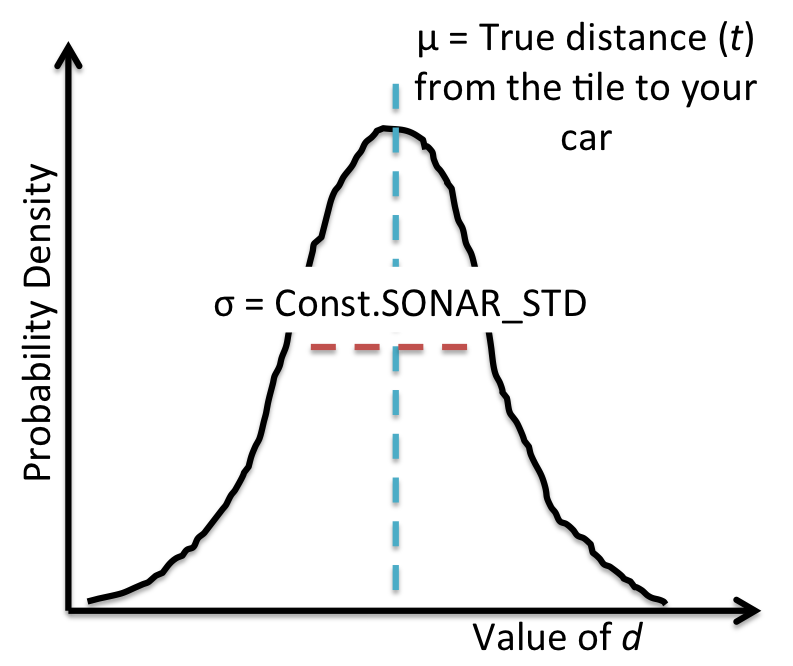
\includegraphics[width=60mm]{images/pdf.png}
\end{center}


\section*{Problem 1 : Emission Probabilities}
In this problem, we assume that the single other car is stationary (e.g., $C_t =
C_{t-1} = C$ for all time steps $t$).
We'll denote the single variable representing the other car's stationary location as $C$,
and note that $p(C)$ is a known local conditional distribution.
You will implement a function \texttt{observe} that upon observing a new
distance measurement $D_t = d_t$ updates the current posterior probability from
$$\mathbb P(C \mid D_1 = d_1, \dots, D_{t-1} = d_{t-1})$$
to find the posterior for the next time step
$$\mathbb P(C \mid D_1 = d_1, \dots, D_t = d_t) $$
The current posterior probability is stored as \texttt{self.belief} in \texttt{ExactInference}.


\begin{center}
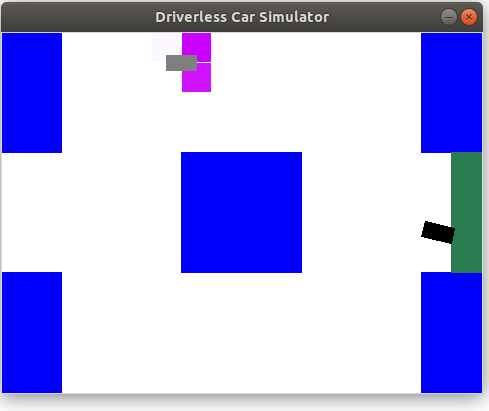
\includegraphics[width=60mm]{images/emission.png}
\end{center}

\begin{enumerate}
    \item[a.] [2 points]     Draw a Bayesian Network describing the distribution of variables 
    
    $C, D_1, D_2, D_3, a_1, a_2, a_3$.
    Shade the variables that have been observed after time step $t=3$, and leave variables that are unobserved unshaded.
     
    \expect{ A drawing of a Bayesian Network with nodes for each variable described above.
    Recall that if $p(X|\text{Parents}(X))$ is a known local conditional distribution, there should be one arrow for each of $X$'s parents
    pointing from the parent to $X$. Hand-drawn or digital drawings are both acceptable, but you need to make sure it is legible.}
    
    \mysolution{
    
    }

    
    \item[b.] [4 points] Give an expression for the joint probability $\mathbb P(C=c, D_1=d_1, D_2=d_2, D_3=d_3)$.
    Your expression should only use known local conditional distributions given by the Bayesian Network.
    Recall that the location of your car at each time step, i.e. $a_1, a_2, a_3$, is known with probability 1.

    \expect{    A mathematical formula for the joint probability distribution of the variables described above that only uses local conditional distributions given in the problem.}

    \mysolution{
    
    }

    \item[c.] [7 points] Now suppose we have previously computed the posterior distribution up through time step t-1, i.e. we know $\mathbb{P}(C|D_1=d_1,...,D_{t-1}=d_{t-1})$. We make a new observation that $D_t=d_t$, and we'd like to update our posterior distribution to $\mathbb{P}(C|D_1=d_1,...,D_t=d_t)$. The unnormalized updated posterior can be computed as:
$\mathbb{P}(C=c|D_1=d_1,..,D_t=d_t)\propto\mathbb{P}(C=c|D_1=d_1,...,D_{t-1}=d_{t-1})p(d_t|C=c)$.


Fill in the observe method in the ExactInference class of submission.py. This method should modify self.belief in place to update the posterior probability of each tile given the observed noisy distance to the other car. After you're done, you should be able to find the stationary car by driving around it (using the flag -p means cars don't move).
\end{enumerate}

%%%%%%%%%%%%%%%%%%%%%%%%%%%%%%%%%%%%%%%%%%%%%%%%%%%%%%%%%%%%%%%%%%%%%%%%%%%%%%%%
\section*{Problem 2 : Transition Probabilities}
Now, let's consider the case where the other car is moving
according to transition probabilities $p(C_{t+1} \mid C_t)$.
We have provided the transition probabilities for you in \texttt{self.transProb}.
Specifically,
\texttt{self.transProb[(oldTile, newTile)]} is the probability of the other car
being in \texttt{newTile} at time step $t+1$ given that it was in \texttt{oldTile} at time step $t$.
\begin{enumerate}

    \item[a.] [2 points]    Draw a Bayesian Network describing the distribution of variables 
    
    $C_1, C_2, C_3, D_1, D_2, D_3, a_1, a_2, a_3$.
  Shade the variables that have been observed after time step $t=3$, and leave variables that are unobserved unshaded.

     
    \expect{A drawing of a Bayesian Network with nodes for each variable described above.
    Recall that if $p(X|\text{Parents}(X))$ is a known local conditional distribution, there should be one arrow for each of $X$'s parents
    pointing from the parent to $X$. Hand-drawn or digital drawings are both acceptable, but you need to make sure it is legible.}
    
    \mysolution{
    
    }

    
    \item[b.] [4 points]   Give an expression for the joint probability $\mathbb P(C_1=c_1, C_2=c_2, C_3=c_3, D_1=d_1, D_2=d_2, D_3=d_3)$ which uses \textit{only} known local conditional distributions.
  Recall that the location of your car at each time step, i.e. $a_1, a_2, a_3$, is known with probability 1.
 
    \expect{A mathematical formula for the joint probability distribution of the variables described above that only uses local conditional distributions given in the problem.}

    \mysolution{
    
    }   

     \item[c.] [7 points] Now, you will implement a function elapseTime that updates the conditional probability about the location of the car at a current time t $\mathbb{P}(C|D_1=d_1,...,D_{t}=d_{t})$ to the next time step t+1 conditioned on the same evidence, via the recurrence:\\
     \begin{equation}
         \begin{aligned}
             & \mathbb{P}(C_{t+1}=c_{t+1}|D_1=d_1,...,D_{t}=d_{t}) \\ 
             & \propto \sum_{c_t}\mathbb{P}(C_t=c_t|D_1=d_1,...,D_{t}=d_{t})p(c_{t+1}|c_t)
         \end{aligned}
     \end{equation}

     This recurrence describes that the probability that the car is at $c_{t+1}$ can be decomposed into all of the locations it could have been located at in the previous timestep ($c_{t}$) weighted by the probability the car would move from $c_{t}$ to $c_{t+1}$.
     
     Again, the posterior probability is stored as self.belief in ExactInference. Finish ExactInference by implementing the elapseTime method. When you are all done, you should be able to track a moving car well enough to drive autonomously by running the following.

     \texttt{python drive.py -a -d -k 1 -i exactInference}
    
\end{enumerate}
%%%%%%%%%%%%%%%%%%%%%%%%%%%%%%%%%%%%%%%%%%%%%%%%%%%%%%%%%%%%%%%%%%%%%%%%%%%%%%%%
\section*{Problem 3 : Which car is it?}


So far, we have assumed that we have a distinct noisy distance reading for each car, but in
reality, our microphone would just pick up an undistinguished set of these signals, and we
wouldn't know which distance reading corresponds to which car.
First, let's extend the notation from before: let $C_{ti} \in \mathbb R^2$ be the location
of the $i$-th car at the time step $t$, for $i = 1, \dots, K$ and $t = 1, \dots, T$.
Recall that all the cars move independently according to the transition dynamics as before.\\


Let $D_{ti} \in \mathbb R$ be the noisy distance measurement of the $i$-th car at time step $t$,
which is now not directly observed.
Instead, we observe the unordered set of distances
$\{ D_{t1}, \dots, D_{tK} \}$ as a collective and so cannot attribute any individual measurement in this set to a specific car.  (For simplicity, we'll assume that all distances are distinct values.)
In other words, you can think of this scenario as the same as observing the list $\mathbf{E_t} = [E_{t1}, \dots, E_{tK}]$
which is a uniformly random permutation of the (noisy) correctly ordered distances $\mathbf{D_t} = [D_{t1}, \dots, D_{tK}]$ where index $i$ represents the noisy distance to car $i$ at time $t$.\\

For example, suppose $K=2$ and $T = 2$.
Before, we might have gotten distance readings of $8$ and $4$ for the first car and
$5$ and $7$ for the second car at time steps $1$ and $2$, respectively.
Now, our sensor readings would be permutations of $\{8, 5\}$ (at time step $1$) and $\{4, 7\}$ (at time step $2$).
Thus, even if we knew the second car was distance $5$ away at time $t = 1$,
we wouldn't know if it moved further away (to distance $7$) or closer (to distance $4$) at time $t = 2$.\\

Here is a diagram that shows the flow of information corresponding to the above situation for the case where $K = 2$ and only showing two timesteps, $t$ and $t+1$. Note that because the observed distances $\mathbf{E_t}$ are a permutation of the true distances $\mathbf{D_t}$, each $E_{ti}$ depends on all of the $D_{ti}$. Also note that the above diagram is not a Bayes net as $E_{t1}$ and $E_{t2}$ are not conditionally independent given $D_{t1}$ and $D_{t2}$ (however, $D_{t1}$ and $D_{t2}$ are conditionally independent given $C_{t1}$ and $C_{t2}$)



\begin{center}
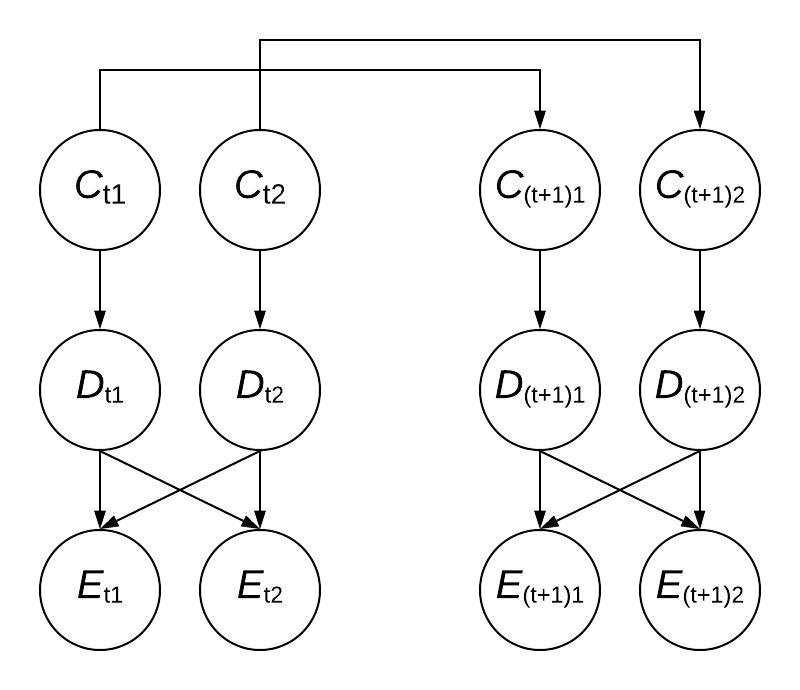
\includegraphics[width=60mm]{images/Q4_diag.jpeg}
\end{center}
%%%%%%%%%%%%%%%%%%%%%%%%%%%%%%%%%%%%%%%%%%%%%%%%%%%  a
  \begin{enumerate}
  \item[a.] [5 points] Suppose we have $K=2$ cars and one time step $T=1$.
    Write an expression for the conditional probability
    $p(C_{11} = c_{11}, C_{12} = c_{12} \mid \mathbf{E_1} = \mathbf{e_1})$
    as a function of the PDF of a Gaussian $ p_{\mathcal N}(v; \mu, \sigma^2)$
    and the prior probability $p(c_{11})$ and $p(c_{12})$ over car locations.
    Your final answer should not contain variables $D_{11}$, $D_{12}$.\\
    
    You can consider $p_{\mathcal N}(v; \mu, \sigma^2)$ as the probability of a Gaussian random variable with mean $\mu$ and standard deviation $\sigma$ having a value $v$.\\
  
  \hint{for $K=1$, the answer would be:
  
  $$p(C_{11} = c_{11} \mid \mathbf{E_1} = \mathbf{e_1}) \propto p(c_{11}) p_{\mathcal N}(e_{11}; \|a_1 - c_{11}\|_2, \sigma^2).$$

where $a_t$ is the position of your car (that you are controlling) at time $t$. Remember that $C_{ti}$ is the position of the $i$th observed car at time $t$. To better inform your use of Bayes' rule, you may find it useful to draw the Bayesian network and think about the distribution of $\mathbf{E_t}$ given $D_{t1}, \dots, D_{tK}$.\\}

\hint{Note that the observed variable(s) are the shuffled/randomized distances $\mathbf{E_t}  = [E_{t1}, E_{t2}, ..., E_{tK}]$.
        These are a random permutation of the unobserved noisy distances $\mathbf{D_t} = [D_{t1}, D_{t2}, ..., D_{tK}]$, where $D_{t1}$ is the distance of car $1$ at timestep $t$.
        Note that $E_{t1}$ is the emission from one of the cars at timestep $t$, but we aren't sure which one (it is NOT necessarily car 1, it could be any of the cars).
        On the other hand, $D_{t1}$ is the measured distance of car 1 (we know with certainty that it comes from car 1), the only issue is that we don't observe it directly.
} %TODO

\hint{To reduce notation, you may write, for example, $p(c_{11}\mid e_{11})$ instead of $p(C_{11}=c_{11} \mid E_{11}=e_{11})$.}

\expect{A mathematical expression, with the steps you took to derive that expression, relating (can be proportionality) $p(C_{11} = c_{11}, C_{12} = c_{12} | \mathbf{E_1} = \mathbf{e_1})$ with the PDF of a Gaussian and the priors $p(c_{11})$ and $p(c_{12})$ over car locations. It may simplify your calculations if you create a proportional expression, similar to the hint for K=1.}


\mysolution{

}
    

%%%%%%%%%%%%%%%%%%%%%%%%%%%%%%%%%%%%%%%%%%%%%%%%%%%% b
\newpage
  \item[b.] [4 points] Assuming the prior $p(c_{1i})$ of where the cars start out is the same for all $i$ (i.e. for all K cars),
    show that the number of assignments for all $K$ cars $(c_{11}, \dots, c_{1K})$
    that obtain the maximum value of
    $p(C_{11} = c_{11}, \dots, C_{1K} = c_{1K} \mid \mathbf{E_1} = \mathbf{e_1})$ is at least $K!$ (K factorial).
    You can also assume that the car locations that maximize the probability above
    are unique ($C_{1i} \neq c_{1j}$ for all $i \neq j$).

\hint{The priors $p(c_{1i})$ are a probability distribution over the possible starting positions ($t=1$) of each car $i$. Note that even if the car positions share the same prior, it doesn't necessarily mean they have the exact same start positions $c_{1i}$ because the start positions are sampled from the prior distribution, which can yield different values each time it is sampled from. However, you should think about what the priors all being the same means intuitively in terms of how we can associate observations with cars.}
      
\note{Note: you don't need to produce a complicated proof for this question. It is acceptable to provide a clear explanation based on your intuitive understanding of the scenario.}

\expect{Either a short mathematical argument or concise explanation for why the statement defined in the problem is true.}

\mysolution{

}

%%%%%%%%%%%%%%%%%%%%%%%%%%%%%%%%%%%%%%%%%%%%%%%%%%%%%%%%%%%%%%%%%%%%%%%%%%%%%%%%
\newpage
\section*{Problem 4: Ethics in Advanced Technologies}

\begin{enumerate}

\item[a.] [3 points] 
Dual-use technologies serve two purposes: one with positive consequences and one with negative consequences. Researchers developing dual-use technologies face a moral dilemma: though they may intend to improve only peaceful, socially beneficial use of the technology, any improvements they make may also aid others who use the technology for harm. For example, tracking of the kind developed in this assignment can be used both in self-driving cars or in surveillance-tracking and autonomous weapons systems, such as lethal drones. To learn more about dual use technologies, refer back to the Externalities and Dual Use Technologies module \href{https://www.youtube.com/watch?v=2xQLCXqOtdU&t=23s}{video}, \href{https://stanford-cs221.github.io/spring2025-extra/modules/search/externalities-and-dual-use-technologies.pdf}{pdf}.

When integrating tracking technologies into self-driving cars, we have to make decisions regarding the tradeoff between the accuracy of the tracking technology and the privacy of the other cars and people on the road. These decisions impact the ways in which the tracking technology might be misused for negative aims. The microphone sensor used in Problems 1-3 preserves privacy relatively well; it only gives us a noisy distance reading. However, in practice, self-driving cars often use cameras (which provide more accurate readings than microphones), but also collect lots of visual information including, but not limited to, pedestrians’ faces and license plate numbers of other vehicles. 

How might the data collected by a camera sensor and/or the output of its reading be misused? What measures, if any, could you take to preempt this misuse? 

\expect{
    In 4-6 sentences, describe a potential misuse of the car tracking technology considered and what measures you might take to preempt such misuse, or explain why there are no such measures.
}

\mysolution{

}

\item[b.] [3 points] Self-driving cars and tracking technologies can potentially be hacked by bad actors to purposefully cause unsafe behavior (e.g., to harm people within a specific community). Research on adversarial ML focuses on how attacks like these can be carried out against machine learning systems and how to develop safeguards against such attacks. Two specific examples of adversarial ML attacks on self-driving cars include:
\begin{itemize}
\item "Cloaking and stealthy attacks" to hide the presence of another vehicle from being detected
\item Sensor deception to make it seem like vehicles are closer or farther than they actually are
\end{itemize}
Let's look at a case study with a sensor deception attack.

Assume that sensor deception affects the problem setup from Problem 1 as follows. The observed distance $D'_{t}$ after attack (see below) is now a skewed Gaussian distribution. To apply skewness, apply the adjustment below to the observed distance variable in submission.py ExactInferenceWithSensorDeception.observe() (we are using a technique called Box-Muller transform but you don’t need to know the details of this method for this problem). The skewness factor is set in the \_\_init\_\_ constructor with a default value of 0.5 (and you can assume the factor will always be greater than 0). Implement this change in the code and rerun python drive.py -a -p -d -k 3 -i exactInferenceWithSensorDeception to observe any changes.

$D'_t = \frac{1}{(1 + \text{skewness}^2)}*D_t + \sqrt{2 * \frac{1}{(1 + \text{skewness}^2)}}$

\expect{Update the code in submission.py observe() for class ExactInferenceWithSensorDeception.}



\item[c.] [2 points] Comment on how one can guard against sensor deception if the type of attack is known beforehand (hint: consider redundancy of sensors).

\expect{
    In 1-2 sentences, describe a way of guarding against sensor deception.
}

\mysolution{

}
\item[d.] [2 points]
One way of increasing security and preventing adversarial attacks is by keeping data on-device. Assume that we are now using particle filtering, which is a more efficient, Monte-Carlo based method for car tracking. Though exact inference works well for small maps, it can be too slow on large worlds such as lombard. With particle filtering, the complexity of the program is $O(numParticles)$ as opposed to $O(numTiles)$. We have filled out the code for particle filtering for you. Simply run \begin{verbatim}python drive.py -a -d -k 3 -i particleFilter\end{verbatim} to observe the behavior. The colors around the other cars represent the belief cloud of those cars’ locations (e.g. purple, green, etc). Comment on how the simulation looks different from the exact inference case and provide a reason why.

\begin{center}
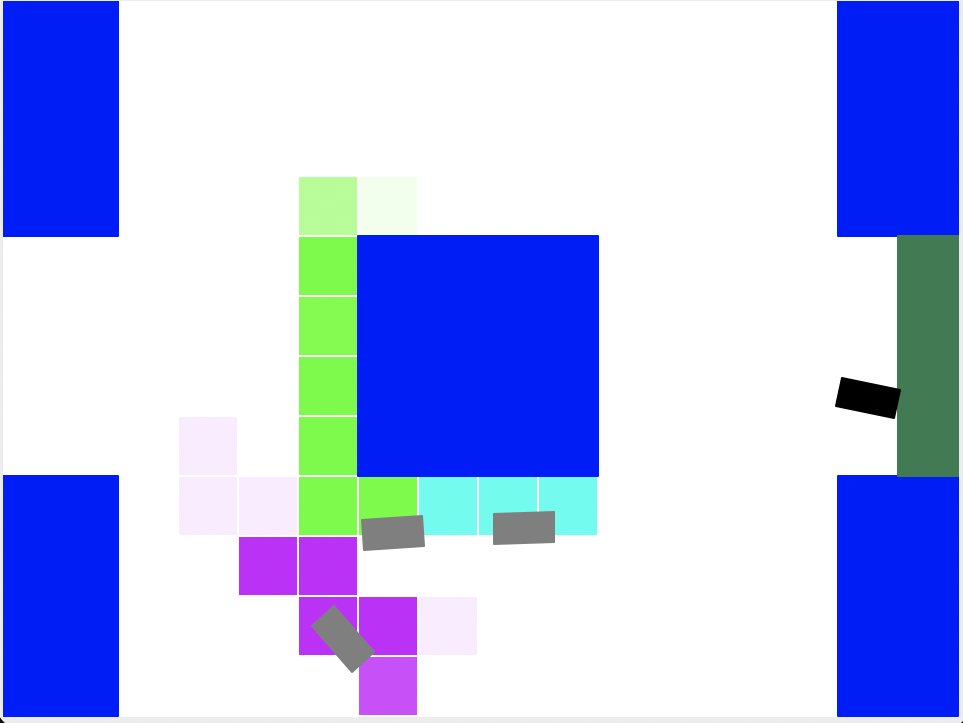
\includegraphics[width=60mm]{images/cloud.png}
\end{center}

\expect{
    In 1-2 sentences, comment on the differences in the simulation with exactInference and particleFilter, and provide a reason why.
}

\mysolution{

}

\item[e.] [2 points]
Assume that because particle filtering is more efficient, we can run the model on-device (vs. exact inference which requires us to run the model in the cloud). By keeping all of the relevant data on-device, we improve the privacy (security) of the data, but decrease the accuracy of the model. While the car can still sometimes make its way down Lombard effectively, it has a less accurate picture of other car locations. How would you weigh this trade-off?

\expect{
    In 3-5 sentences, discuss how you would evaluate the privacy accuracy trade-off outlined above.
}

\mysolution{

}

\item[f.] [2 points]
Watch this week's \href{https://drive.google.com/file/d/1Ti5d5qv5_b-PfeyA4ZSUK4rVzhW_rh9-/view}{embedded ethics lecture}. Suppose we have a camera-based autonomous vehicle that can be further trained on customers' anonymized camera data. Name an adversarial attack, a potential impact it could have on the vehicle, and a mitigation for that attack.

\expect{
    In 3-5 sentences, discuss an example of an adversarial attack, how it could impact the vehicle, and a mitigation for the attack.
}

\mysolution{

}

\end{enumerate}


\end{enumerate}

\end{document}
